% Session 3 -- the SSH chain: the same bulk, two dimerizations, two spectra.
% Placement: sec. "The SSH model", after the dangling-site paragraph.
% Rendered by figures/blender/s03f03_ssh.py, labels in figures/overlays/s03f03_ssh.tex.
\begin{aqmfigure}{fig:s03:ssh}{The Su-Schrieffer-Heeger chain, drawn with the same eight sites and
the same unit cells in both rows, which are the translucent slabs, so that the only difference is
which of the two bonds is the strong one, drawn as the thick rod. Next to each chain is its
spectrum, the eigenvalues of the open chain in units of the strong hopping. (a) In front, the
intracell hopping dominates, $t\gg1$ (here $t=4$). Every site is paired into a dimer, and the levels
form two groups around $\pm t$, spread a little by the weak hopping, with a clear gap around zero,
which is the trivial phase. (b) Behind, the intercell hopping dominates, $t\to0$ (here $t=1/4$). The
dimer pattern is shifted by one site and the first and last sites, the two glowing ones, are left
uncoupled. The same bulk spectrum now has two extra states at $E=0$, the two short rods in the gap,
one localized at each end, which is the topological phase. The two chains cannot be distinguished
in the bulk, and the difference is only at the ends, which is what a bulk invariant has to predict.
At small but finite $t$ the two end states hybridize through the chain, and their splitting away
from zero is only exponential in the chain length. For $t=1/4$ and eight sites the two levels sit
at $\pm0.004$, which is too small to see at this scale.}
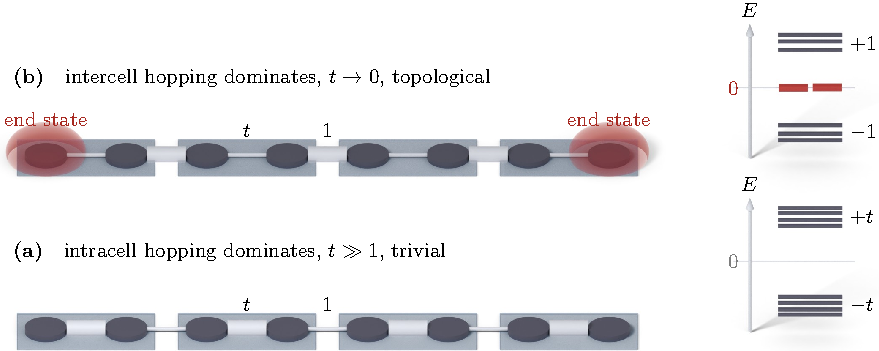
\includegraphics{figures/pdf/s03f03_ssh.pdf}
\end{aqmfigure}
